\documentclass{article}
\usepackage{mathtools}
\usepackage{amsmath}
\usepackage{graphicx}
\begin{document}
	\section*{Lsg Vorschlag A+N Ü010 Maximilian Maag}
	\section*{Aufgabe A}
	Gleichungen für Niveaulinien ergibt mehrere unterschiedlich Große Kreise um den Ursprung. Körpger Kegel. \\ \\
	\includegraphics[width=\linewidth, height=\linewidth]{10A}
	\section*{Aufgabe B}
	$f(x,y) = x^7 * y^2$ \\
	$f_x = 7x^6 * y^2$ \\
	$f_y = x^7 * 2y$ 
	\subsection*{a)}
	\[grad(f) = \begin{pmatrix}
		7x^6 * y^2 \\ x^7 * 2y
	\end{pmatrix}
	 \]
	\[grad(f) = \begin{pmatrix}
		28 \\ 4
	\end{pmatrix}\] \\
	\[\begin{pmatrix}
		28 \\ 4
	\end{pmatrix} = \sqrt{28^2 + 4^2} = 20\sqrt{2} \]
	\subsection*{b)}
	Skalarprodukt bilden: \\ \\
	\section*{Aufgabe 1}
	\subsection*{a)}
	$f(x,y) = 3x + 6y$ \\
	$c = 3x + 6y$ \\
	$c - 3x = 6y$ \\
	$f(x) = -\frac{3}{6}x + \frac{c}{6}$ \\
	$f(0) = -\frac{3}{6}x + \frac{0}{6}$ \\
	$f(0) = -\frac{3}{6}x$ \\
	$f(-6) = -\frac{3}{6}x - 1$ \\
	$f(6) = f(0) = -\frac{3}{6}x + 1$ \\
	$f(-12) = -\frac{3}{6}x - \frac{12}{6}$ \\
	$f(-12) = -\frac{3}{6}x - 2$ \\
	$f(12) = -\frac{3}{6}x + \frac{12}{6}$ \\
	$f(12) = -\frac{3}{6}x + 2$ \\ \\
	Es handelt sich um eine Ebene. \\
	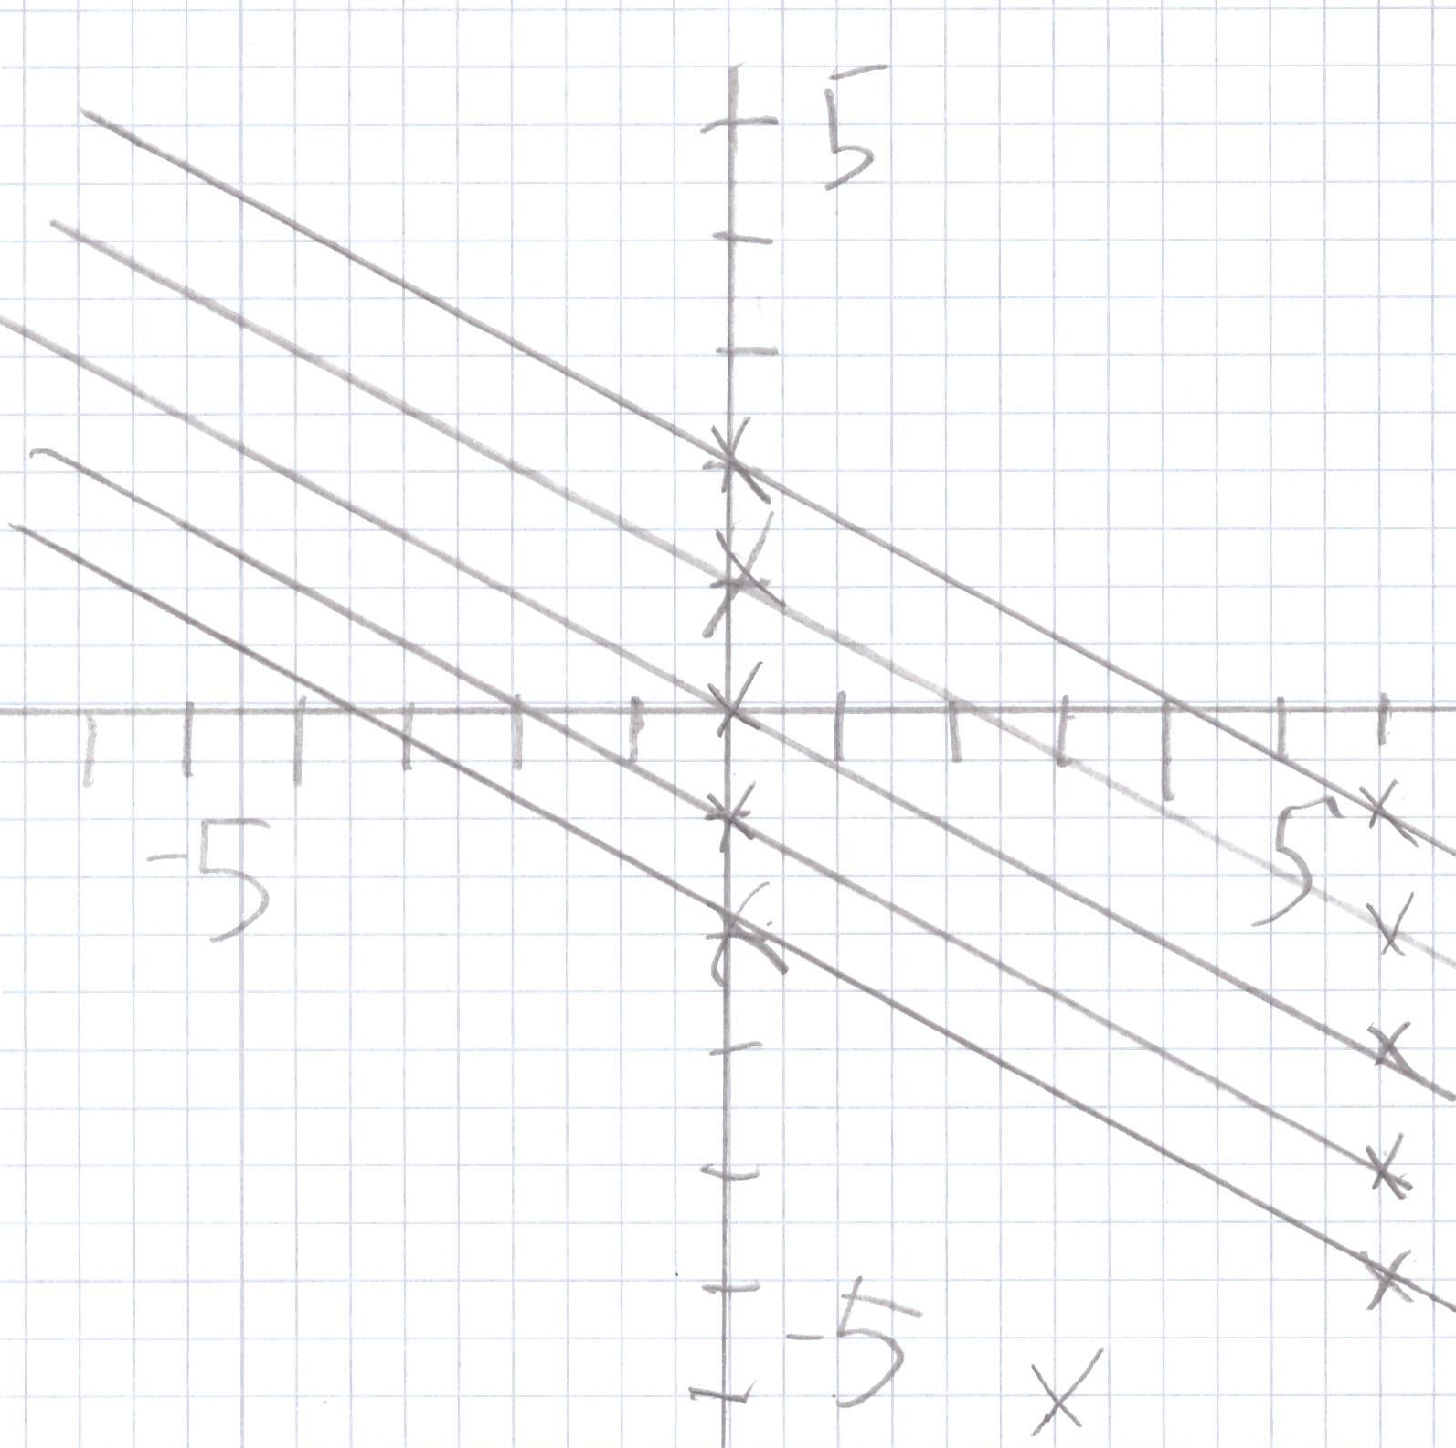
\includegraphics[width=\linewidth]{101a}
	
	\subsection*{b)}
	$f(x, y) = x^2+ y^2–2y$ \\
	$x^2+ y^2–2y = 0$ \\ \\
	$x^2 + y^2 - 2y = 3$ \\ \\
	$x^2 + y^2 - 2y = 8$ \\ \\
	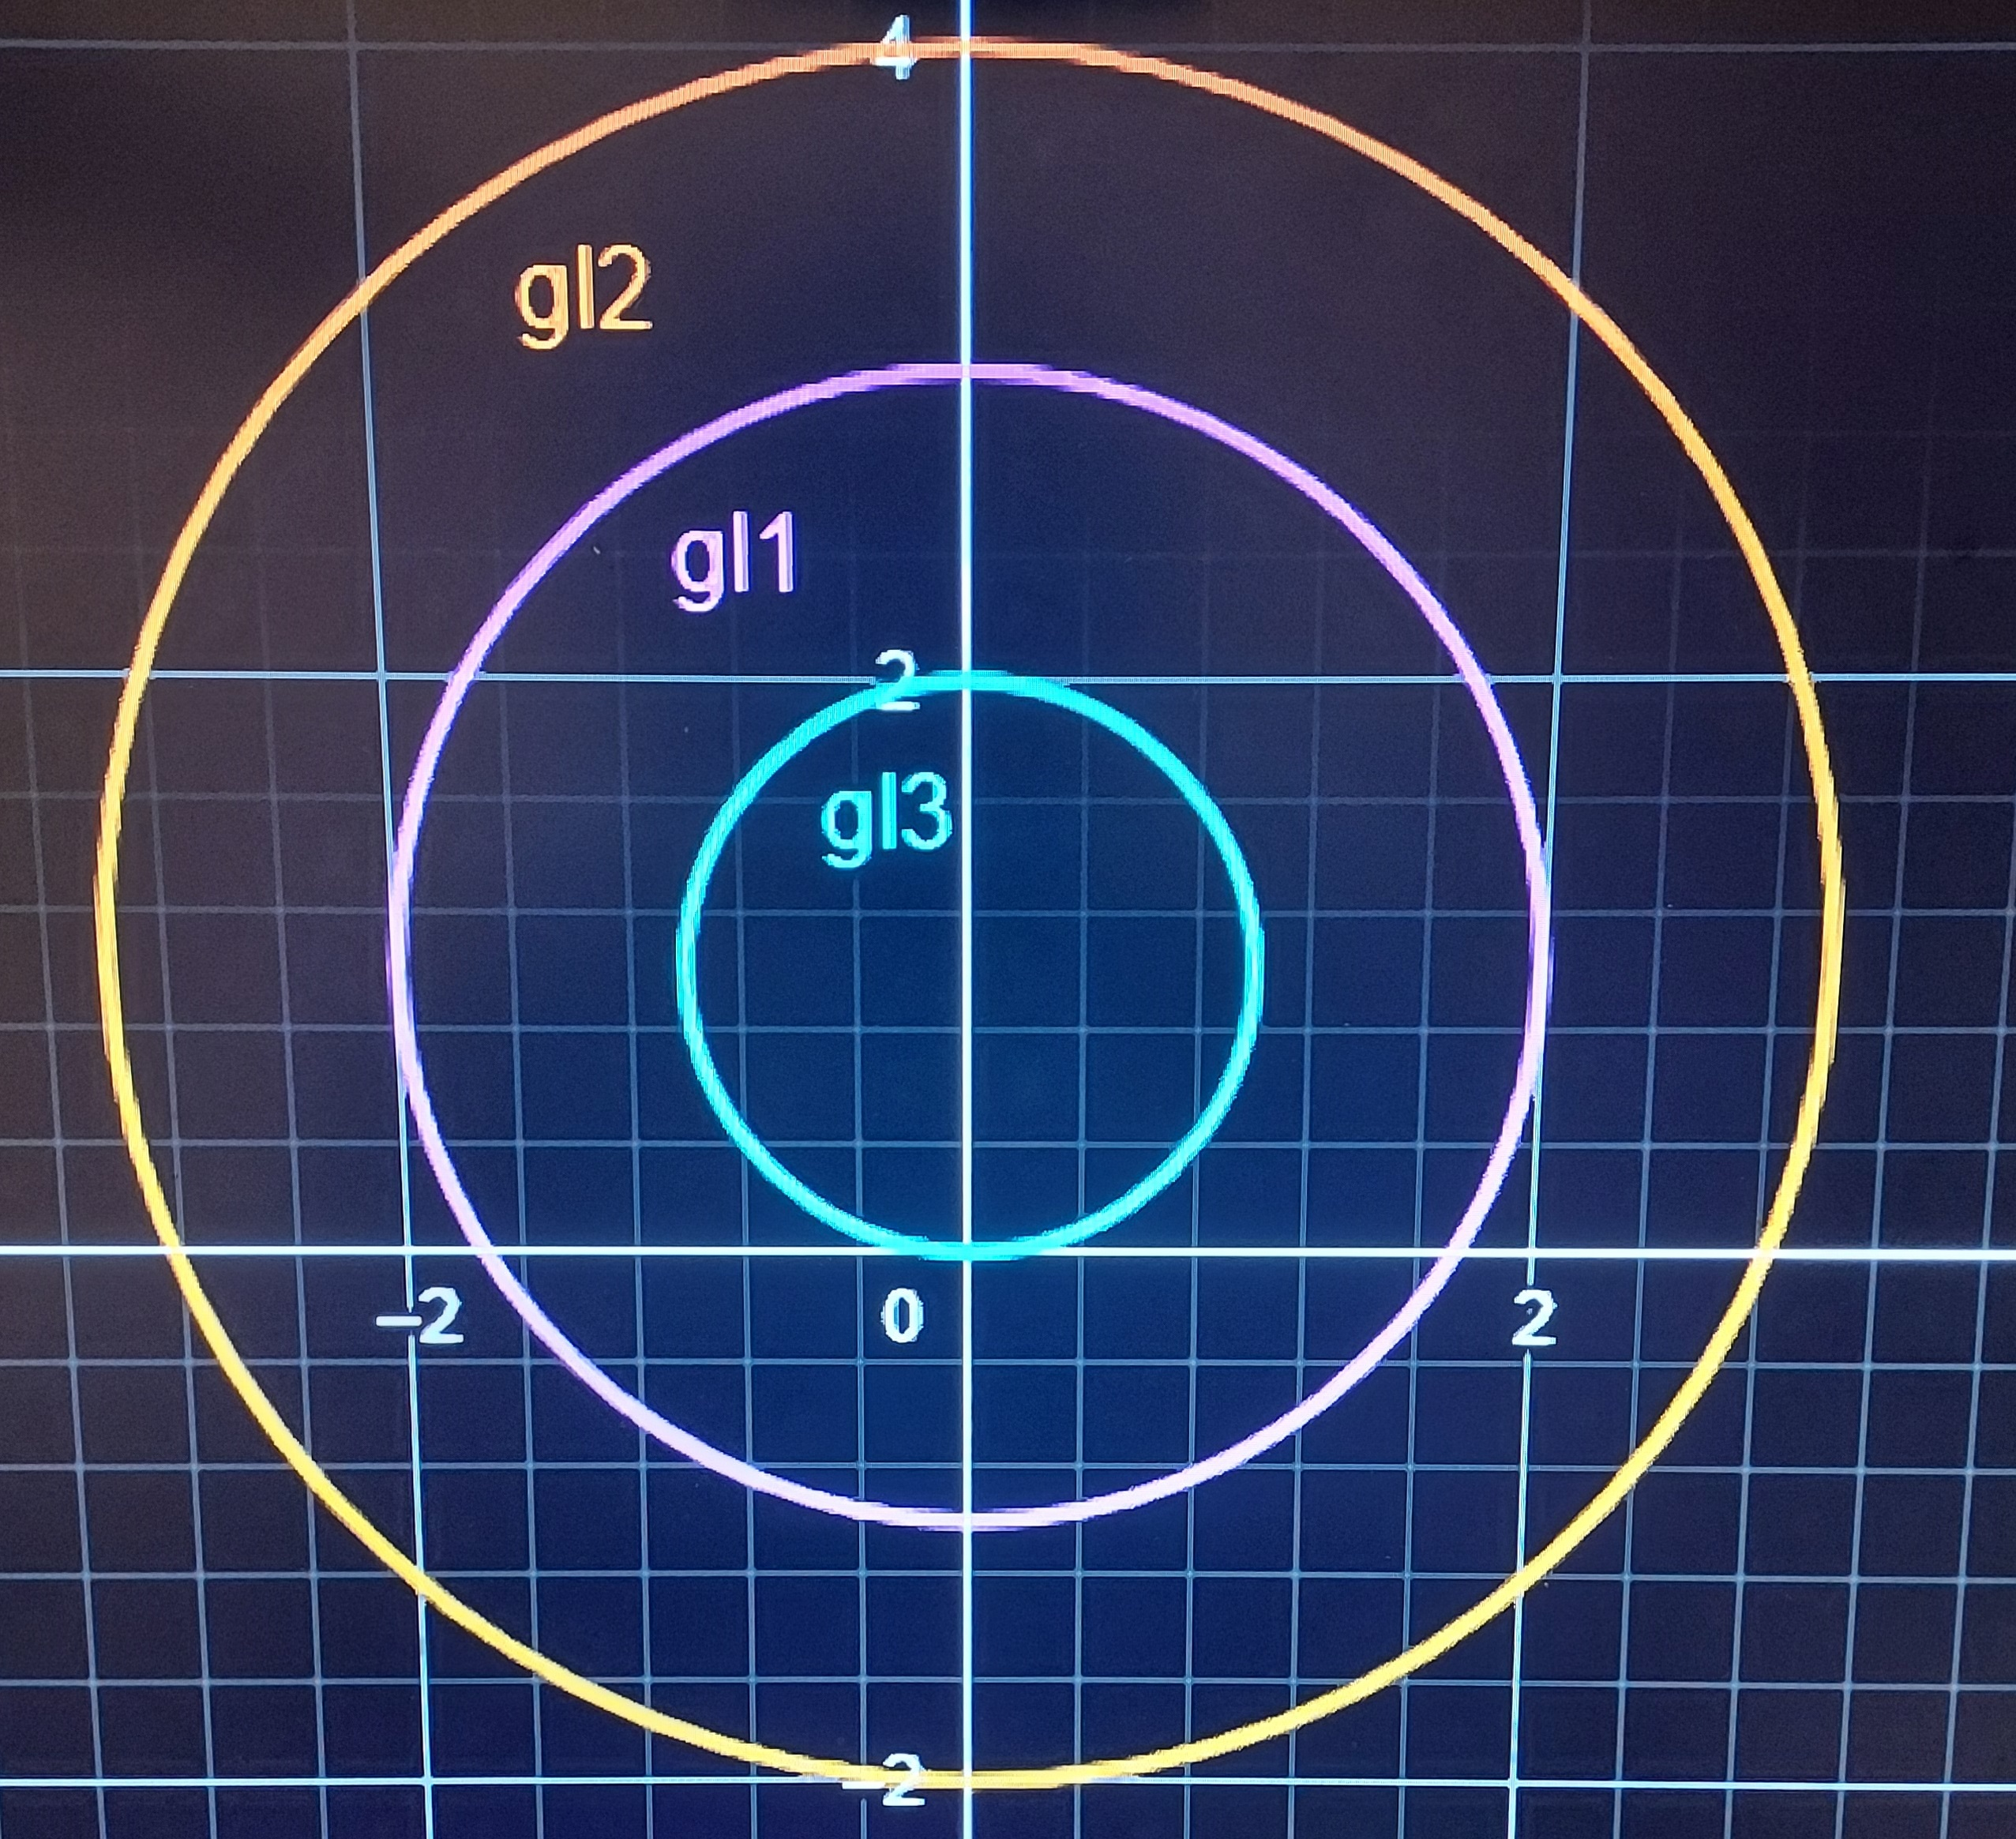
\includegraphics[width=\linewidth]{101b} \\
	Verschobener Kreis.
	\section*{Aufgabe 2}
	$f(x,y) = x^3 * y^4$ \\
	$f_x = 3x^2 * y^4$; $f_y = x^3 * 4y^3$ \\
	$g(x,y) = 1 + 3(x-1) + 4(y - 1)$ \\
	$g(x,y) = 1 + 3x - 3 + 4y - 4$ \\
	$g(x,y) = 3x +  4y -6$ \\
	\section*{Aufgabe 3}
	\subsection*{a)}
	$c = \sqrt{1 - x^2 - y^2}$ \\
	$c^2 = 1 - x^2 - y^2$ \\
	$c^2 - 1 = -x^2 - y^2$ \\
	$-c^2 + 1 = x^2 + y^2$ \\
	$1 = x^2 + y^2$ \\
	$-(0,2)^2 + 1 = x^2 + y^2$ \\
	$0,96 = x^2 + y^2$ \\
	$-(0,6)^2 + 1 = x^2 + y^2$ \\
	$0,64 = x^2 + y^2$ \\
	$-(0,8)^2 + 1 = x^2 + y^2$ \\
	$0,36 = x^2 + y^2$ \\
	$0 = x^2 + y^2$ \\ \\
	\includegraphics[width=\linewidth]{103a}
	\subsection*{b)}
	Tangentialebene an der Stelle $(\frac{1}{3}, \frac{2}{3})$ \\
	$f(x,y) = \sqrt{1 - x^2 - y^2}$ \\
	$f(x,y) = (1 - x^2 - y^2)^{\frac{1}{2}}$ \\
	$f_x = -\frac{1}{2}(1 - x^2 - y^2)^{\frac{1}{2}}*2x$ \\
	$f_y = -\frac{1}{2}(1 - x^2 - y^2)^{\frac{1}{2}}*2y$ \\ \\
	$g(x,y) = f(x_0,y_0) + f_x(x_0,y_0)(x - x_0) + f_y(x_0,y_0)(y - y_0)$ \\ \\
	$f(x,y) = \sqrt{1 - \frac{1}{3}^2 - \frac{2}{3}^2}$ \\
	$f(x,y) = \sqrt{\frac{4}{9}}$ \\
	$f(x,y) = \frac{2}{3}$ \\
	$f_x(x,y) = -\frac{1}{2}$; $f_y(x,y) = -1$ \\
	$g(x,y) = \frac{2}{3}  -\frac{1}{2}(x - \frac{1}{3}) -1(y - \frac{2}{3})$ \\
	$g(x,y) = \frac{2}{3}  -\frac{1}{2}x + \frac{1}{6} -y + \frac{2}{3}$ \\
	$g(x,y) = -\frac{1}{2}x  -y + \frac{3}{2}$ \\
\end{document}